\documentclass[english]{article}
\usepackage{graphicx}
\usepackage[margin=.8in]{geometry}
\usepackage{float}
\usepackage{hyperref}
\hypersetup{
    colorlinks=true,
    linkcolor=blue,
    filecolor=blue,      
    urlcolor=blue,
}

\begin{document}

\title{ User Manual \\
	\large For Pascal to Mips Compiler}
\author{Joseph Miller}
\maketitle

\section{Using the compiler}

Below is a series of steps in order to take your Pascal code and create mips assembly code.

\begin{enumerate}
   \item Open the command prompt or terminal on your computer
   \item Navigate to the directory that contains Compiler.jar
   \item Enter the following into the command line: \textbf{java -jar Compiler.jar pascalfile.pas}
\end{enumerate}

\noindent There should be three new files in the directory that Compiler.jar was run in. If not, reference section \ref{errors}

\begin{itemize}
   \item  \textit{pascalfilename.asm} : the compiled assembly code
   \item  \textit{pascalfilename.table} : the symbol table of variables delacred
   \item  \textit{pascalfilename.tree}: syntax tree of the pascal code
\end{itemize}

\noindent The .asm can be run in \href{http://spimsimulator.sourceforge.net/}{QtSpim} - a simulator for MIPs assembly code. The interface can be seen below.

\begin{figure}[H]
\begin{center}
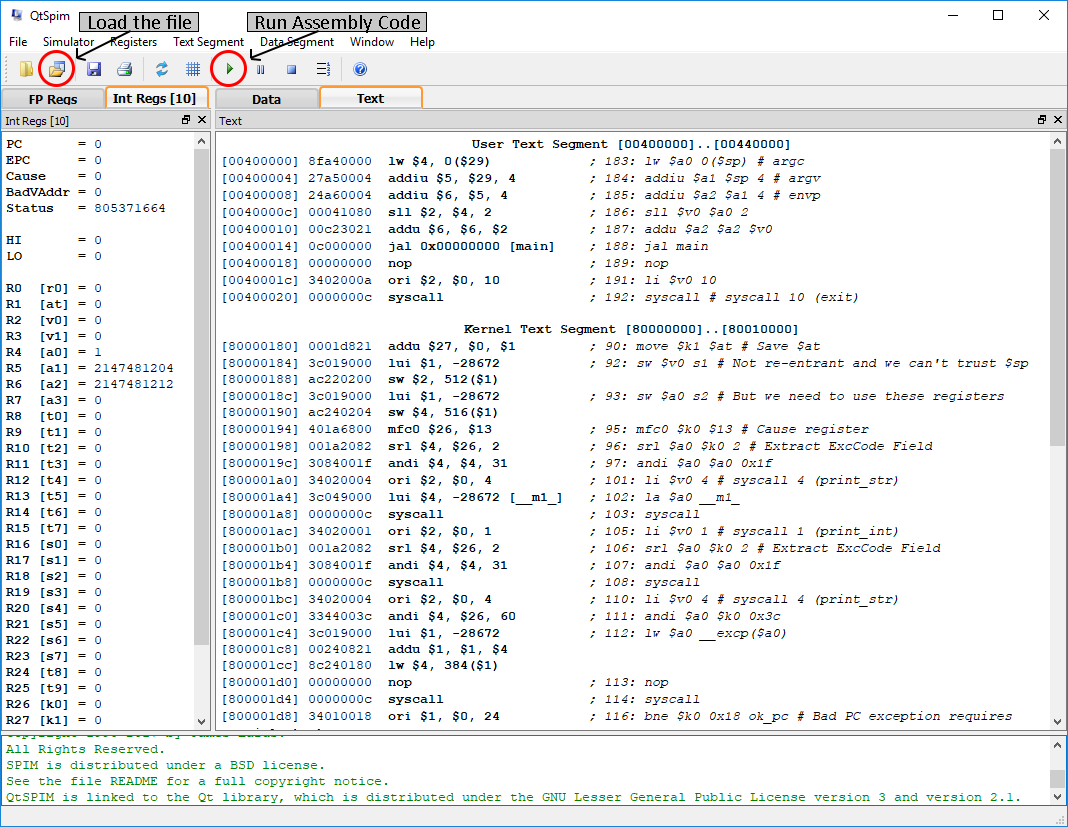
\includegraphics[width=.8\textwidth]{qtspim.PNG}
\end{center}
\caption{\label{QtSpim}QtSpim Interface}
\end{figure}


\section{Error Handling} \label{errors}








\end{document}